%!TEX root = ../dokumentation.tex

\chapter{Stand der Technik}

In diesem Kapitel werden bereits vorhandene Technologien, die im Kontext dieser Arbeit von Bedeutung sind, vorgestellt und evaluiert.

\section{Datengeneratoren}

Es gibt bereits einige Applikationen, die in der Lage sind, Daten nach Modellen zu generieren; diese sind jedoch stark auf einen bestimmten Anwendungsfall zugeschnitten.

\begin{itemize}
    \item \textbf{Scikit-Learn} \cite{scikit-learn:paper, scikit-learn:generator}: Die \ac{ML}-Bibliothek scikit-learn bietet Funktionalitäten, um Beispieldaten zu generieren. Allerdings bietet sie nur vorgefertigte Funktionen, die bestimmte Muster zufällig generieren. Die Funktionen lassen sich kaum anpassen und es ist nicht möglich, damit ein komplexes Modell abzubilden.
    \begin{figure}[H]
        \centering
        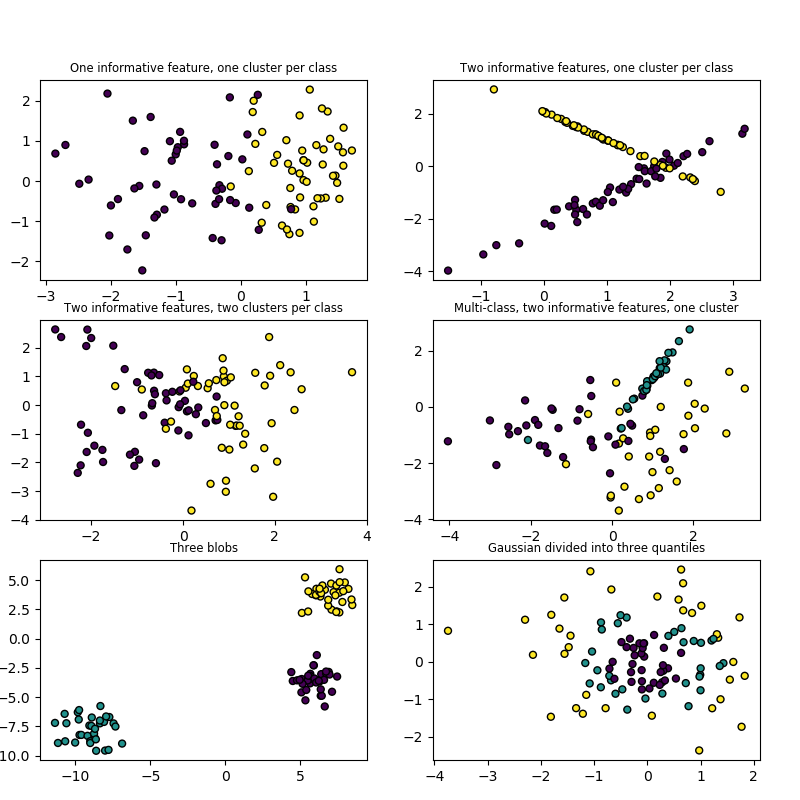
\includegraphics[width=0.5\textwidth]{sklearn_random_dataset.png}
        \caption{Durch scikit-learn generierte Daten \cite{scikit-learn:plots}}
        \label{fig:sklearndata}
    \end{figure}
    \item \textbf{SynthOSNdataGenerator} \cite{synthosndatagenerator}: Dieses Programm ist in der Lage, die Struktur eines sozialen Netzwerks zu erzeugen. Auch hier ist die Funktionalität sehr auf den Anwendungsfall angepasst und nicht universell genug, um als Basis für die in dieser Arbeit zu entwickelnde Applikation zu dienen.
    \item \textbf{log-synth} \cite{logsynth}: Das Tool log-synth ist in der Lage, künstliche Log-Dateien zu erzeugen. Es erlaubt eine sehr flexible Konfiguration und hat bereits viele eingebaute Funktionen, jedoch ist es schwierig, Zusammenhänge zwischen mehreren Eigenschaften zu modellieren. Dadurch kann auch dieses Tool nicht als Grundlage für die Arbeit genommen werden.
\end{itemize}

Da keine dieser Applikationen in der Lage ist, die Anforderungen dieser Arbeit abzudecken, muss eine neue Applikation entwickelt werden.

\section{Node Editor}

Eine der Anforderungen ist die Benutzung einer grafischen Oberfläche zur Modellierung des Modells zur Datengenerierung. Dafür wurde entschieden, das \textit{\ac{DFP}} Konzept umzusetzen.

Beim \ac{DFP} wird das Programm in einem gerichteten Graphen dargestellt. Jeder Knoten bildet eine Funktion ab und hat Ein- und Ausgabeschnittstellen. Über die Eingabeschnittstellen erhält die Funktion des Knotens die benötigten Parameter; das Resultat der Funktion wird über die Ausgabeschnittstellen anderen Knoten zur Verfügung gestellt. Die Schnittstellen von Knoten können über Kanten verbunden werden. Kanten symbolisieren einen Datenfluss von einer Aus- zu einer Eingabeschnittstelle \cite{dataflow}. Einer der Vorteile von \ac{DFP} ist, dass Abhängigkeiten von Operationen durch die grafische Programmierung direkt ersichtlich sind. Auch sind Programme, die mit \ac{DFP} erstellt wurden, parallelisierbar, solange die Knoten bei der Berechnung keine Seiteneffekte haben \cite{dataflow}.

Der Node-Editor ist die grafische Oberfläche, die es erlaubt, das \ac{DFP}-Programm zu bearbeiten. Technisch gesehen ist ein Node-Editor ein Editor für gerichtete Graphen. Es hat sich aber bei Anwendersoftware der Begriff \textit{Node-Editor} durchgesetzt \cite{nodeeditor:blender, nodeeditor:maya}. Deshalb werden in dieser Arbeit die Begriffe \textit{Node-Editor} und \textit{Graph-Editor} synonym verwendet.

Für die Entwicklung des Node-Editors wird eine Möglichkeit benötigt, grafische Elemente an beliebigen Positionen anzeigen zu können. Dafür gibt es zwei Ansätze.

Die eine Möglichkeit ist die Nutzung von klassischen \ac{HTML}-Elementen wie \texttt{<div>} und der Anwendung der \ac{CSS}
-Eigenschaft \texttt{position: absolute}. Mit dieser Eigenschaft können Elemente innerhalb des Elternelements frei verschoben werden \cite{mdn:position}. Zusätzlich können mit dieser Methode auch \ac{SVG} verwendet werden, um komplexe Formen wie beispielsweise die Verbindungen zwischen den Knoten zu zeichnen.

Die andere Möglichkeit ist die Nutzung des HTML5-Canvas. Der Canvas ist ein HTML-Element, das verwendet wird, um Grafiken auf einer Webseite zu zeichnen. Gezeichnet wird mittels JavaScript über die Canvas-Programmierschnittstelle \cite{mdn:canvas}.

Zwar bietet der Canvas eine hohe Leistung, er hat aber einen für diese Arbeit gravierenden Nachteil: Es können keine existierenden \ac{HTML}-Steuerelemente wie Eingabefelder oder Buttons verwendet werden. Alle Steuerelemente müssen selber gezeichnet werden. Zusätzlich muss auch die Logik der Steuerelemente selber implementiert werden. Beispielsweise muss bei einem Tastendruck in einem Textfeld der entsprechende Buchstabe an der Position des Cursors eingefügt werden.

\subsection{Node-Editoren für JavaScript}

Aufgrund der in Kapitel \ref{sec:anforderungsanalyse} (S. \pageref{sec:anforderungsanalyse}) beschriebenen Anforderungen wurden folgende Kriterien entwickelt, die der Node-Editor unbedingt bieten muss:
\begin{itemize}
    \item Steuerelemente in den Knoten, um komplexe Werte einzustellen
    \item Steuerelemente in den Eingangsschnittstellen, damit konstante Werte an nicht verbundenen Eingangsschnittstellen direkt eingestellt werden können
    \item Sidebar für sehr komplexe Einstellungen von Knoten, wie zum Beispiel einer eigenen Wahrscheinlichkeitsdichtefunktion
    \item Ausführliche Dokumentation, um eigene Knoten und Erweiterungen umsetzen zu können
\end{itemize}

Es gibt bereits einige offene Bibliotheken für JavaScript, die die Funktionalität eines Node-Editors bieten. Im Folgenden werden einige dieser Bibliotheken vorgestellt.

\begin{itemize}
    \item \textbf{litegraph.js} ist eine Canvas-basierte Bibliothek. Damit bietet sie eine hohe Leistung. Es ist allerdings aufwändig, eigene Steuerelemente einzufügen, da diese selber gezeichnet werden müssen. Auch ist die Dokumentation spärlich. \cite{litegraph}
    \item \textbf{ThreeNodes.js} ist auf die Bearbeitung von WebGL-Szenen ausgelegt. Die Bibliothek basiert auf HTML und SVG und bietet laut eigener Aussage eine einfache Schnittstelle, um neue Knoten hinzuzufügen. Leider gibt es keine Dokumentation, außerdem wurde das Projekt zuletzt im Mai 2016 aktualisiert. \cite{threenodes}
    \item \textbf{vue-blocks} ist eine rudimentäre Umsetzung eines Node-Editors mit Vue.js. Vue.js ist ein Frontend-Framework für JavaScript, welches in Kapitel \ref{sec:baklava:ui} (S. \pageref{sec:baklava:ui}) vorgestellt wird. Die Möglichkeiten von vue-blocks sind allerdings sehr beschränkt; es gibt beispielsweise keine Möglichkeit, eigene Steuerelemente in den Nodes anzuzeigen. \cite{vueblocks}
    \item \textbf{Nodes} ist eine mit Vue.js entwickelte Bibliothek, die auf dem HTML5-Canvas aufbaut. Der Autor schreibt allerdings selber, dass die Bibliothek als Experiment gedacht war und eher eine eigene Bibliothek entwickelt werden solle statt diese Bibliothek zu verwenden. \cite{nodes}
    \item \textbf{Linker} baut auf HTML und SVG auf. Leider ist es mit Linker nicht möglich, Steuerelemente in die Nodes einzufügen. \cite{linker}
\end{itemize}

Da keine der Bibliotheken alle der oben genannten Kriterien erfüllt, wurde entschieden, eine eigene Bibliothek zu entwickeln. Diese vereint die Vorteile der vorgestellten Bibliotheken und wird in Kapitel \ref{sec:grapheditor} (Seite \pageref{sec:grapheditor}) näher vorgestellt. Dabei wurde entschieden, nicht auf den HTML5-Canvas zu setzen, da dies einen sehr hohen Implementierungsaufwand mit sich bringen würde.